\documentclass[../Bitcoin Blink.tex]{subfiles}
\graphicspath{{\subfix{../assets/images/}}}
\begin{document}
\subsection{Messaging}
\begin{figure}[h]
\begin{center}
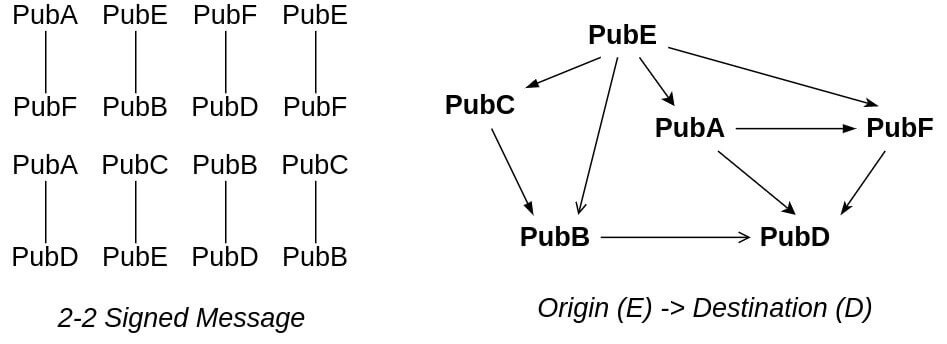
\includegraphics[width=8cm]{topology}
\caption{Topology}
\label{topology}
\end{center}
\end{figure}
Delivery of unconfirmed transactions to nodes plays an important role in finality. Shared mempools defile the network with duplicated data, resulting in a poor choice of transactions by accepting higher fees to include in a block. A direct-messaging system should be deployed with messaging instructions specific to each party as opposed to gossip protocols. Paths are attached with unconfirmed transactions directly from the constructed network graph, which is available to all nodes with public keys as pseudonymous identities protecting privacy. Two peering parties mutually sign a 2–2 random message for every $x$ blocks (ring size) and are gossiped across the network to identify the connection as online. All the signed random messages prove that each pubkey signature can display a network topology map (see Fig.\ref{topology}) from a node's point of reference. Paths are encrypted end-to-end with routing \cite{poon2016bitcoin} instructions so that the origin cannot be traced. Nodes route transactions to the destinations where producers can attach the transaction to their allocated block. Since the stake information is available in the public ledger, client wallets can construct transactions along with path information that routes to the nearest blocks for instant finality. Transactions are always atomic, providing a solution to queuing issues. Responsibilities are provided to all participants, where nodes only receive the transactions that they need to include, and client wallets should construct shorter paths to provide the best user experience.
\end{document}
